\phantomsection
\setcounter{secnumdepth}{3}

\setcounter{chapter}{1}
\chapter[{PHÂN TÍCH VÀ THIẾT KẾ HỆ THỐNG TÁC NHÂN}]{Phân tích và Thiết kế Hệ thống Tác nhân}

Chương này đặc tả từng thành phần của hệ thống, bắt đầu bằng tổng quan pipeline end-to-end để người đọc hiểu mục đích của từng phần trước khi đọc chi tiết.

\section{Tổng quan pipeline end-to-end}

\begin{figure}[H]
    \centering
    \begin{tikzpicture}[node distance=1.8cm, >=stealth, every node/.style={font=\small}]
        \node[draw, rounded corners, align=center, minimum width=3.0cm, minimum height=0.9cm, fill=blue!12] (pcgnn) {PCGNN sinh\\bản đồ};
        \node[draw, rounded corners, align=center, right of=pcgnn, xshift=2.2cm, minimum width=3.0cm, minimum height=0.9cm, fill=blue!12] (bfs) {BFS kiểm tra +\\phân loại dễ/khó};
        \node[draw, rounded corners, align=center, right of=bfs, xshift=2.2cm, minimum width=3.0cm, minimum height=0.9cm, fill=blue!12] (tile) {TilemapGenerator\\curriculum};
        \node[draw, rounded corners, align=center, right of=tile, xshift=2.2cm, minimum width=3.0cm, minimum height=0.9cm, fill=orange!18] (agent) {CombatAgent\\quan sát};
        \node[draw, rounded corners, align=center, right of=agent, xshift=2.2cm, minimum width=3.0cm, minimum height=0.9cm, fill=green!18] (ppo) {PPO cập nhật\\chính sách};
        \draw[->] (pcgnn) -- (bfs);
        \draw[->] (bfs) -- (tile);
        \draw[->] (tile) -- (agent);
        \draw[->] (agent) -- (ppo);
        \draw[->, dashed, bend right=30] (ppo.south) to node[below, font=\scriptsize]{episode mới} (tile.south);
    \end{tikzpicture}
    \caption{Pipeline huấn luyện end-to-end. Các khối xanh là hệ thống sinh bản đồ; khối cam là quan sát; khối xanh lá là thuật toán học.}
    \label{fig:pipeline_overview}
\end{figure}

Luồng hoạt động: PCGNN chạy ngoại tuyến để sinh tập bản đồ đa dạng; BFS lọc bản đồ hợp lệ và chia theo độ khó; TilemapGenerator nạp bản đồ đúng mức vào từng lesson curriculum; CombatAgent thu vector quan sát từ Unity và chuyển hành động về game; PPO cập nhật chính sách dựa trên phần thưởng. Mỗi phần dưới đây đặc tả một khối trong hình này.

\section{Mô hình hóa bài toán dưới dạng MDP}

Theo mô hình học tăng cường đã trình bày ở Chương~1, bài toán được mô tả dưới dạng một Quy trình Quyết định Markov (Markov Decision Process -- MDP) với bộ thành phần $(S,A,P,R,\gamma)$ \cite{Schulman2017}. Tại mỗi bước quyết định, tác nhân quan sát trạng thái hiện tại $s_t$, chọn hành động $a_t$, nhận phần thưởng $r_t$, sau đó môi trường Unity cập nhật sang trạng thái $s_{t+1}$ theo logic gameplay, vật lý 2D và cách sinh bản đồ.

Trong phạm vi khóa luận, $S$ là không gian quan sát vector của CombatAgent; $A$ là không gian hành động rời rạc nhiều nhánh gồm bốn nhánh; $R$ là hàm thưởng kết hợp giữa tín hiệu kết quả như tiêu diệt kẻ địch và tín hiệu định hình như tiếp cận mục tiêu; $\gamma=0.99$ là hệ số chiết khấu trong cấu hình PPO. Mục tiêu huấn luyện là tìm chính sách $\pi_{\theta}(a|s)$ tối đa hóa kỳ vọng tổng thưởng:

\begin{equation}
    J(\pi_\theta) = \mathbb{E}_{\tau \sim \pi_\theta}
    \left[\sum_{t=0}^{T}\gamma^t r_t\right].
\end{equation}

Điểm khó của bài toán nằm ở chỗ phân phối trạng thái thay đổi theo từng episode. Bản đồ được chọn từ nhiều text map khác nhau, vị trí sinh có thể cố định hoặc ngẫu nhiên theo lesson, kẻ địch và đạn di chuyển liên tục, còn phần thưởng hoàn thành phòng chỉ xuất hiện khi tác nhân tiêu diệt đủ mục tiêu. Vì vậy, hệ thống cần một biểu diễn trạng thái đủ giàu để mô tả chiến đấu, nhưng vẫn đủ gọn để học hiệu quả bằng PPO.

\section{Không gian quan sát}

Hệ thống sử dụng quan sát dạng vector thay vì ảnh pixel. Lựa chọn này giúp giảm chi phí mẫu, tránh phải học lại các đặc trưng thị giác cơ bản, đồng thời phù hợp với mục tiêu nghiên cứu là đánh giá ảnh hưởng của curriculum learning và các kỹ thuật khám phá trên một môi trường có cấu trúc. Trong Unity Inspector, kích thước quan sát vector của behavior CombatAgentConfig được cấu hình là 207 chiều.

\begin{table}[H]
    \centering
    \small
    \caption{Cấu trúc vector quan sát 207 chiều của CombatAgent}
    \label{tab:obs_207}
    \begin{tabular}{|p{4cm}|c|p{8cm}|}
        \hline
        \textbf{Nhóm quan sát} & \textbf{Số chiều} & \textbf{Nội dung chính} \\
        \hline
        Trạng thái người chơi & 13 & Máu, đạn, hồi chiêu, trạng thái sẵn sàng của vũ khí, tốc độ, sát thương gần đây, hướng vận tốc và giá trị đệm để giữ kích thước cố định. \\
        \hline
        Thông tin toàn cục & 4 & Tỷ lệ kẻ địch nhìn thấy, tỷ lệ đạn nhìn thấy, thời gian episode đã chuẩn hóa và tín hiệu chết gần đây. \\
        \hline
        Kẻ địch gần nhất & 54 & 3 kẻ địch $\times$ 18 đặc trưng: vị trí tương đối, vận tốc tương đối, khoảng cách, máu, mức đe dọa, trạng thái tấn công, hồi chiêu và giá trị đệm. \\
        \hline
        Đạn trong vùng nhìn & 120 & 10 viên đạn $\times$ 12 đặc trưng: vị trí tương đối, vận tốc, khoảng cách, thời gian ước lượng tới va chạm, loại chủ sở hữu và giá trị đệm. \\
        \hline
        Tường/vật cản & 16 & 16 tia ray đều quanh tác nhân, mỗi tia trả về khoảng cách chuẩn hóa tới tường gần nhất. \\
        \hline
        \textbf{Tổng} & \textbf{207} & $13 + 4 + 54 + 120 + 16 = 207$. \\
        \hline
    \end{tabular}
\end{table}

\begin{figure}[H]
\centering
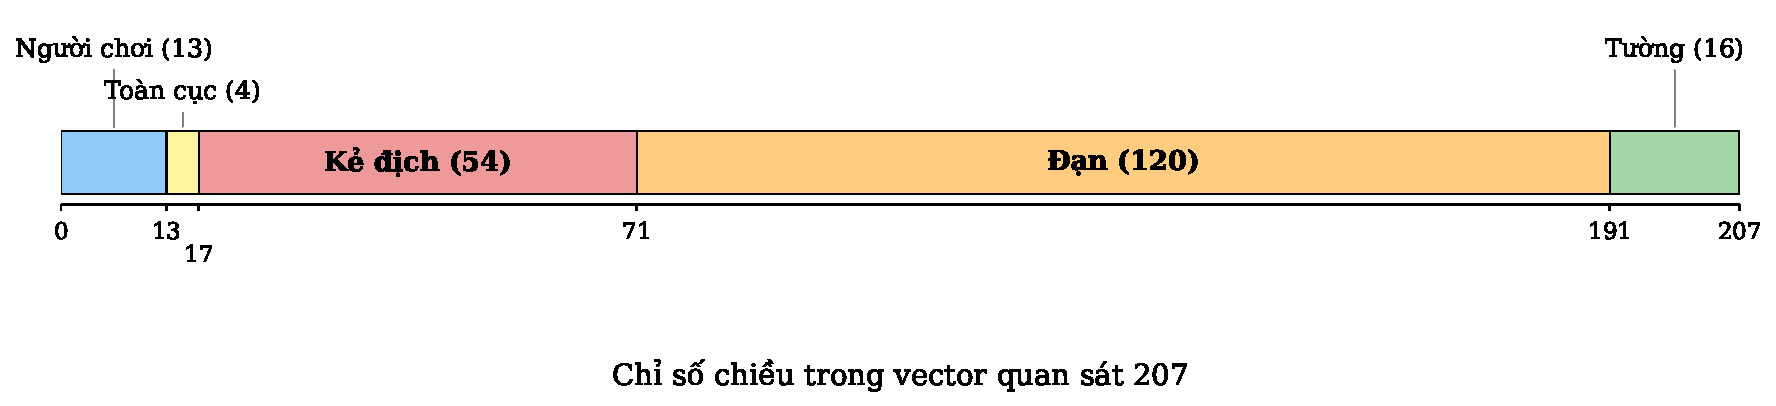
\includegraphics[width=0.95\textwidth]{figures/training/fig_obs_breakdown.pdf}
\caption{Cấu trúc vector quan sát 207 chiều của CombatAgent, phân theo nhóm thông tin. Chiều rộng mỗi đoạn xấp xỉ tỷ lệ với số chiều; nhóm Đạn (120) chiếm hơn nửa vector, tiếp theo là Kẻ địch (54).}
\label{fig:obs_breakdown}
\end{figure}

Thiết kế này cố ý tách rõ thông tin người chơi, kẻ địch, đạn và tường. Tác nhân không cần suy luận vị trí đạn từ ảnh thô, nhưng vẫn phải học cách kết hợp nhiều nguồn nguy cơ: vừa tiếp cận kẻ địch để gây sát thương, vừa tránh đạn và không mắc vào tường. Vì số lượng kẻ địch và đạn trong cảnh chơi có thể thay đổi, các nhóm đặc trưng được giới hạn bởi MaxEnemies=3 và MaxBullets=10; nếu thiếu đối tượng thì hệ thống thêm giá trị 0 để vector luôn có kích thước cố định.

\section{Không gian hành động}

CombatAgent sử dụng không gian hành động rời rạc nhiều nhánh gồm bốn nhánh với kích thước $(3,3,3,9)$. Đây là điểm khác biệt quan trọng so với phiên bản FSM trước đó chỉ chọn một trạng thái cao mức. Thay vì ra lệnh "đang di chuyển" hoặc "đang tấn công" ở mức thô, tác nhân trực tiếp chọn hướng di chuyển, ý định chiến đấu và hướng ngắm.

\begin{table}[H]
    \centering
    \small
    \caption{Không gian hành động rời rạc nhiều nhánh của CombatAgent}
    \label{tab:action_space}
    \begin{tabular}{|c|c|p{9cm}|}
        \hline
        \textbf{Branch} & \textbf{Kích thước} & \textbf{Ý nghĩa} \\
        \hline
        0 & 3 & moveX: không di chuyển theo trục X, sang trái, sang phải. \\
        \hline
        1 & 3 & moveY: không di chuyển theo trục Y, đi xuống, đi lên. \\
        \hline
        2 & 3 & combat: không hành động, tấn công, dash. Các lựa chọn tấn công hoặc dash có thể bị action mask khi vũ khí/kỹ năng chưa sẵn sàng. \\
        \hline
        3 & 9 & aim: giữ hướng cũ hoặc ngắm theo 8 hướng rời rạc. \\
        \hline
    \end{tabular}
\end{table}

\begin{figure}[H]
\centering
\begin{tikzpicture}[
  every node/.style={font=\small},
  rootnode/.style={draw, rounded corners=4pt, fill=orange!25, minimum width=4.0cm, minimum height=0.85cm, align=center},
  branchnode/.style={draw, rounded corners=3pt, minimum width=2.4cm, minimum height=0.85cm, align=center},
  leafbox/.style={draw=gray!55, rounded corners=2pt, minimum width=2.4cm, minimum height=1.55cm, align=center, font=\scriptsize, fill=gray!8},
  totalbox/.style={draw, rounded corners=3pt, fill=yellow!18, minimum width=8.5cm, minimum height=0.7cm, align=center, font=\small},
  >=stealth
]
% Root
\node[rootnode] (root) at (0,0) {Hành động $a_t$\\(multi-discrete, 4 nhánh độc lập)};

% 4 branches
\node[branchnode, fill=blue!15]  (mX) at (-6.0,-1.7) {moveX\\(3)};
\node[branchnode, fill=cyan!18]  (mY) at (-2.0,-1.7) {moveY\\(3)};
\node[branchnode, fill=red!15]   (cb) at ( 2.0,-1.7) {combat\\(3)};
\node[branchnode, fill=green!18] (am) at ( 6.0,-1.7) {aim\\(9)};

\draw[->] (root.south) -- (mX.north);
\draw[->] (root.south) -- (mY.north);
\draw[->] (root.south) -- (cb.north);
\draw[->] (root.south) -- (am.north);

% Leaves
\node[leafbox] (lX) at (-6.0,-3.6) {none\\left\\right};
\node[leafbox] (lY) at (-2.0,-3.6) {none\\down\\up};
\node[leafbox] (lC) at ( 2.0,-3.6) {none\\attack\\dash};
\node[leafbox] (lA) at ( 6.0,-3.6) {hold + 8 hướng:\\N, NE, E, SE,\\S, SW, W, NW};

\draw[->, gray!70] (mX) -- (lX);
\draw[->, gray!70] (mY) -- (lY);
\draw[->, gray!70] (cb) -- (lC);
\draw[->, gray!70] (am) -- (lA);

% Total annotation
\node[totalbox] at (0,-5.0)
  {Tổng tổ hợp: $3 \times 3 \times 3 \times 9 = 243$\quad(81 tổ hợp \emph{di chuyển $\times$ ngắm} nếu bỏ qua combat)};
\end{tikzpicture}
\caption{Cấu trúc cây của không gian hành động $(3,3,3,9)$ của CombatAgent. Bốn nhánh được chọn độc lập tại mỗi bước, tạo 243 tổ hợp tổng cộng trước khi áp dụng action mask. Riêng tổ hợp di chuyển (9 hướng) $\times$ ngắm (9 hướng) đã đạt 81 trạng thái điều khiển.}
\label{fig:action_space_tree}
\end{figure}

Tổ hợp hai nhánh moveX và moveY tạo ra 9 hướng di chuyển (bao gồm đứng yên), trong khi nhánh aim điều khiển hướng tấn công. Entropy cực đại lý thuyết của không gian hành động, nếu mọi lựa chọn đều hợp lệ và phân phối đều, là:

\begin{equation}
    H_{\max} = \ln(3) + \ln(3) + \ln(3) + \ln(9) \approx 5.49 \text{ nat}.
    \label{eq:max_entropy}
\end{equation}

Giá trị này được dùng lại trong Chương~4 khi phân tích hiện tượng entropy plateau. Lưu ý là action mask có thể làm entropy cực đại thực tế thấp hơn tại một số trạng thái, vì các hành động như tấn công hoặc dash không phải lúc nào cũng hợp lệ.

\section{Thiết kế hàm phần thưởng}

Hàm thưởng kết hợp phần thưởng kết quả thưa và phần thưởng định hình dày \cite{Ibrahim2024}. Nhóm phần thưởng kết quả thưa phản ánh mục tiêu thật của phòng chơi, còn phần thưởng định hình cung cấp tín hiệu học trung gian để PPO không bị kẹt trong giai đoạn chưa từng hoàn thành phòng.

\begin{table}[H]
    \centering
    \small
    \caption{Các thành phần thưởng chính trong hai phiên bản hàm thưởng}
    \label{tab:reward_components}
    \begin{tabular}{|p{4.4cm}|c|c|p{5.2cm}|}
        \hline
        \textbf{Sự kiện} & \textbf{v1} & \textbf{v2} & \textbf{Vai trò} \\
        \hline
        Gây sát thương & $+1.0$ & $+1.5$ & Khuyến khích gây sát thương thay vì chỉ né tránh. \\
        \hline
        Hạ một kẻ địch & $+3.0$ & $+5.0$ & Tín hiệu kết quả thưa nhưng có ý nghĩa chiến thuật cao. \\
        \hline
        Dọn sạch toàn bộ phòng & $+5.0$ & $+10.0$ & Mục tiêu cuối của episode; reward v2 tăng mạnh tín hiệu hoàn thành. \\
        \hline
        Tiếp cận mục tiêu & $+0.008 \times \Delta d$ & $+0.003 \times \Delta d$ & Định hình theo khoảng cách, giảm ở v2 để tránh tác nhân chỉ tối ưu hành vi tiếp cận. \\
        \hline
        Tấn công đúng hướng & $+0.05$ & $+0.15$ & Tăng phần thưởng cho ý định tấn công có căn chỉnh tốt. \\
        \hline
        Đứng gần địch không hành động & $-0.0005$ & $-0.002$ & Phạt hành vi chần chừ trong vùng nguy hiểm. \\
        \hline
        Tác nhân chết & $-2.0$ & $-2.0$ & Tín hiệu kết thúc âm. \\
        \hline
    \end{tabular}
\end{table}

Bảng~\ref{tab:reward_components} chỉ liệt kê các thành phần chính. Trong hiện thực, mã nguồn còn có các tín hiệu nhỏ hơn như phạt theo thời gian, phạt nhận sát thương, thưởng dash hữu ích, phạt tấn công không hợp lệ và phần thưởng căn chỉnh hướng ngắm. Cấu hình v1 được dùng cho các run chính từ run34 đến run54. Cấu hình v2 được dùng trong run55 như một thí nghiệm thay đổi thang thưởng, vì vậy các giá trị phần thưởng trung bình của run55 không được so trực tiếp với các run v1.

\section{Sinh bản đồ bằng PCGNN và TilemapGenerator}

Môi trường huấn luyện dùng pipeline hai tầng. Tầng thứ nhất là PCGNN chạy ngoại tuyến ở phía Python để sinh nhiều bản đồ từ một genome đã huấn luyện. Tầng thứ hai là TilemapGenerator trong Unity, có nhiệm vụ đọc các bản đồ văn bản đã được tuyển chọn, chuyển thành tilemap, chọn vị trí sinh và đưa phòng vào episode huấn luyện. Thiết kế này giữ được tính đa dạng của PCGNN nhưng tránh việc gọi Python trực tiếp trong mỗi episode Unity, nhờ đó giảm rủi ro độ trễ và lỗi tích hợp trong quá trình huấn luyện.

NEAT tiến hóa quần thể genome qua nhiều thế hệ; mỗi genome mã hóa một mạng sinh tile. Fitness kết hợp tỷ lệ bản đồ hợp lệ, novelty nội bộ, novelty so với archive và độ phủ MAP-Elites. MAP-Elites chia không gian đặc trưng bản đồ (wall\_ratio, path\_length) thành các ô và lưu generator tốt nhất mỗi ô, ngăn quần thể hội tụ về một kiểu bản đồ duy nhất. Chi tiết cơ chế NEAT và novelty search trong \cite{Beukman2022}.


Mỗi bản đồ sau khi sinh được chuẩn hóa về định dạng văn bản của trò chơi: ký tự \# biểu diễn tường, . biểu diễn sàn, P là vị trí sinh người chơi và E là vị trí sinh kẻ địch. Vì đầu ra của PCGNN chủ yếu là ma trận tile, đề tài bổ sung một bộ chuyển đổi để đặt P/E trên cùng một thành phần liên thông của vùng sàn. Sau đó hệ thống chạy BFS để kiểm tra người chơi có thể đi tới kẻ địch hay không trước khi bản đồ được đưa vào tập huấn luyện.

\begin{figure}[H]
    \centering
    \begin{tikzpicture}[node distance=1.7cm, >=stealth, every node/.style={font=\small}]
        \node[draw, rounded corners, align=center, minimum width=2.7cm, minimum height=0.9cm] (pcgnn) {PCGNN\\genome};
        \node[draw, rounded corners, align=center, right of=pcgnn, xshift=2.0cm, minimum width=2.9cm, minimum height=0.9cm] (adapter) {Bộ chuyển đổi\\text map};
        \node[draw, rounded corners, align=center, right of=adapter, xshift=2.0cm, minimum width=3.0cm, minimum height=0.9cm] (metric) {BFS + chỉ số\\độ khó};
        \node[draw, rounded corners, align=center, below of=adapter, yshift=-0.4cm, minimum width=3.2cm, minimum height=0.9cm] (tiers) {Easy/Medium/Hard\\thư mục};
        \node[draw, rounded corners, align=center, right of=tiers, xshift=2.0cm, minimum width=3.0cm, minimum height=0.9cm] (unity) {TilemapGenerator\\Unity episode};
        \draw[->] (pcgnn) -- (adapter);
        \draw[->] (adapter) -- (metric);
        \draw[->] (metric) -- (tiers);
        \draw[->] (tiers) -- (unity);
    \end{tikzpicture}
    \caption{Luồng sinh và tuyển chọn bản đồ bằng PCGNN trước khi đưa vào Unity}
    \label{fig:map_generation_workflow}
\end{figure}

\begin{figure}[H]
    \centering
    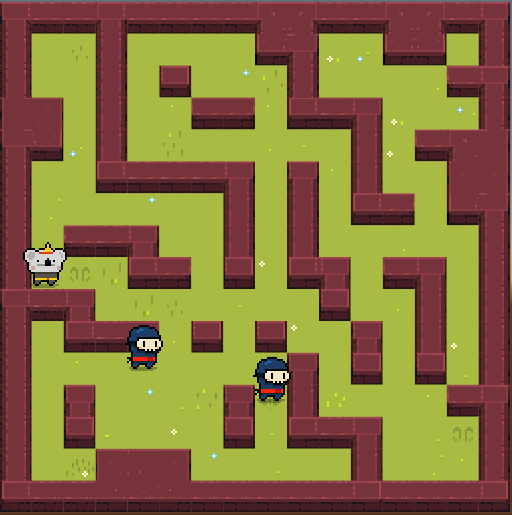
\includegraphics[width=0.72\textwidth]{figures/map_gen.png}
    \caption{Ví dụ bản đồ sau khi được dựng trong môi trường Unity từ text map}
    \label{fig:unity_generated_map_example}
\end{figure}

Độ khó bản đồ được đánh giá bằng các chỉ số hình học gồm tỷ lệ tường, độ dài đường đi ngắn nhất giữa P và E, tỷ lệ ngõ cụt, tỷ lệ vùng có thể đi tới và độ khó A*. Trong phiên bản sử dụng cho tập bản đồ hiện tại, điểm độ khó được tính theo công thức:

\begin{equation}
\begin{aligned}
    \text{difficulty\_score} ={} & 0.90 \times \text{wall\_ratio} + 0.05 \times \min(\text{path\_norm}, 1.0) \\
    & {}+ 0.03 \times \text{dead\_end\_ratio} + 0.02 \times \text{astar\_difficulty}.
\end{aligned}
\label{eq:map_difficulty_score}
\end{equation}

Trong công thức~\ref{eq:map_difficulty_score}, \emph{wall\_ratio} được gán trọng số cao nhất vì mật độ tường ảnh hưởng trực tiếp đến không gian di chuyển và mức độ phức tạp của bản đồ. Các thành phần còn lại như độ dài đường đi, tỷ lệ ngõ cụt và độ khó A* đóng vai trò bổ trợ, giúp tinh chỉnh thứ hạng độ khó thay vì chi phối hoàn toàn kết quả phân loại. Thay vì đặt ngưỡng tuyệt đối cứng cho mọi generator, hệ thống có thể sắp xếp bản đồ theo độ khó tương đối: 5\% dễ nhất được đưa vào Easy, 5\% tiếp theo vào Medium và phần còn lại vào Hard. Cách chia này phù hợp với giai đoạn tuyển chọn thủ công vì người thiết kế vẫn có thể xem lại từng thư mục và chọn những bản đồ tốt nhất trước khi đưa sang Unity.

\textbf{Tập bản đồ đưa vào Unity.} Ở giai đoạn sinh bản đồ ban đầu, tập bản đồ PCGNN chính có 1000 bản đồ kích thước $14\times14$ và có thể chia theo tỷ lệ 5/5/90 để tạo ba nhóm Easy, Medium và Hard. Tuy nhiên, khóa luận không sử dụng toàn bộ 1000 bản đồ này trong Unity. Thay vào đó, các bản đồ được xem xét và chọn lọc theo từng mức độ khó, sau đó chỉ một tập con đại diện được gán trực tiếp cho các thí nghiệm hiện tại, gồm 5 Easy, 5 Medium và 50 Hard. Cách dùng tập con này giúp kiểm soát chất lượng bản đồ trước khi mở rộng phân loại đầy đủ: Easy và Medium đóng vai trò tạo tín hiệu học ban đầu trong giai đoạn đầu, còn Hard là phân phối mục tiêu chiếm phần lớn thời gian huấn luyện.

\begin{table}[H]
    \centering
    \small
    \caption{Phân bố bản đồ đang gán trong Unity theo nhóm độ khó}
    \label{tab:map_split}
    \begin{tabular}{|p{2.5cm}|c|c|p{7.5cm}|}
        \hline
        \textbf{Nhóm} & \textbf{Số bản đồ} & \textbf{Tỷ lệ} & \textbf{Vai trò trong huấn luyện} \\
        \hline
        Easy   & 5  & 8.33\%  & Tạo tín hiệu học ban đầu cho giai đoạn $\sim$0--70k bước; tập nhỏ đã được chọn để tác nhân có cơ hội hoàn thành phòng thường xuyên hơn. \\
        \hline
        Medium & 5  & 8.33\%  & Bước trung gian từ Easy sang Hard, dùng khoảng $\sim$70k--140k bước. \\
        \hline
        Hard   & 50 & 83.33\% & Phân phối mục tiêu, chiếm hơn 95\% thời gian huấn luyện; số lượng lớn hơn hai nhóm đầu để tăng đa dạng bố cục. \\
        \hline
    \end{tabular}
\end{table}

Trong Unity, TilemapGenerator không cần biết bản đồ được vẽ tay hay sinh bằng PCGNN. Thành phần này chỉ đọc text asset theo nhóm hiện tại, dựng tilemap và kiểm tra lại vùng có thể đi tới. Với các lesson dùng fixed spawn, TilemapGenerator ưu tiên ô sàn có độ phủ BFS tốt để tránh trường hợp người chơi hoặc kẻ địch bị cô lập. Với lesson dùng random spawn, người chơi và kẻ địch được chọn từ các ô sàn hợp lệ nhằm tăng phương sai môi trường. Hình~\ref{fig:unity_tilemap_generator_inspector} minh họa cấu hình TilemapGenerator trong Inspector, trong đó Unity đang dùng chế độ Curriculum với 5 bản đồ Easy, 5 bản đồ Medium và 50 bản đồ Hard.

\begin{figure}[H]
    \centering
    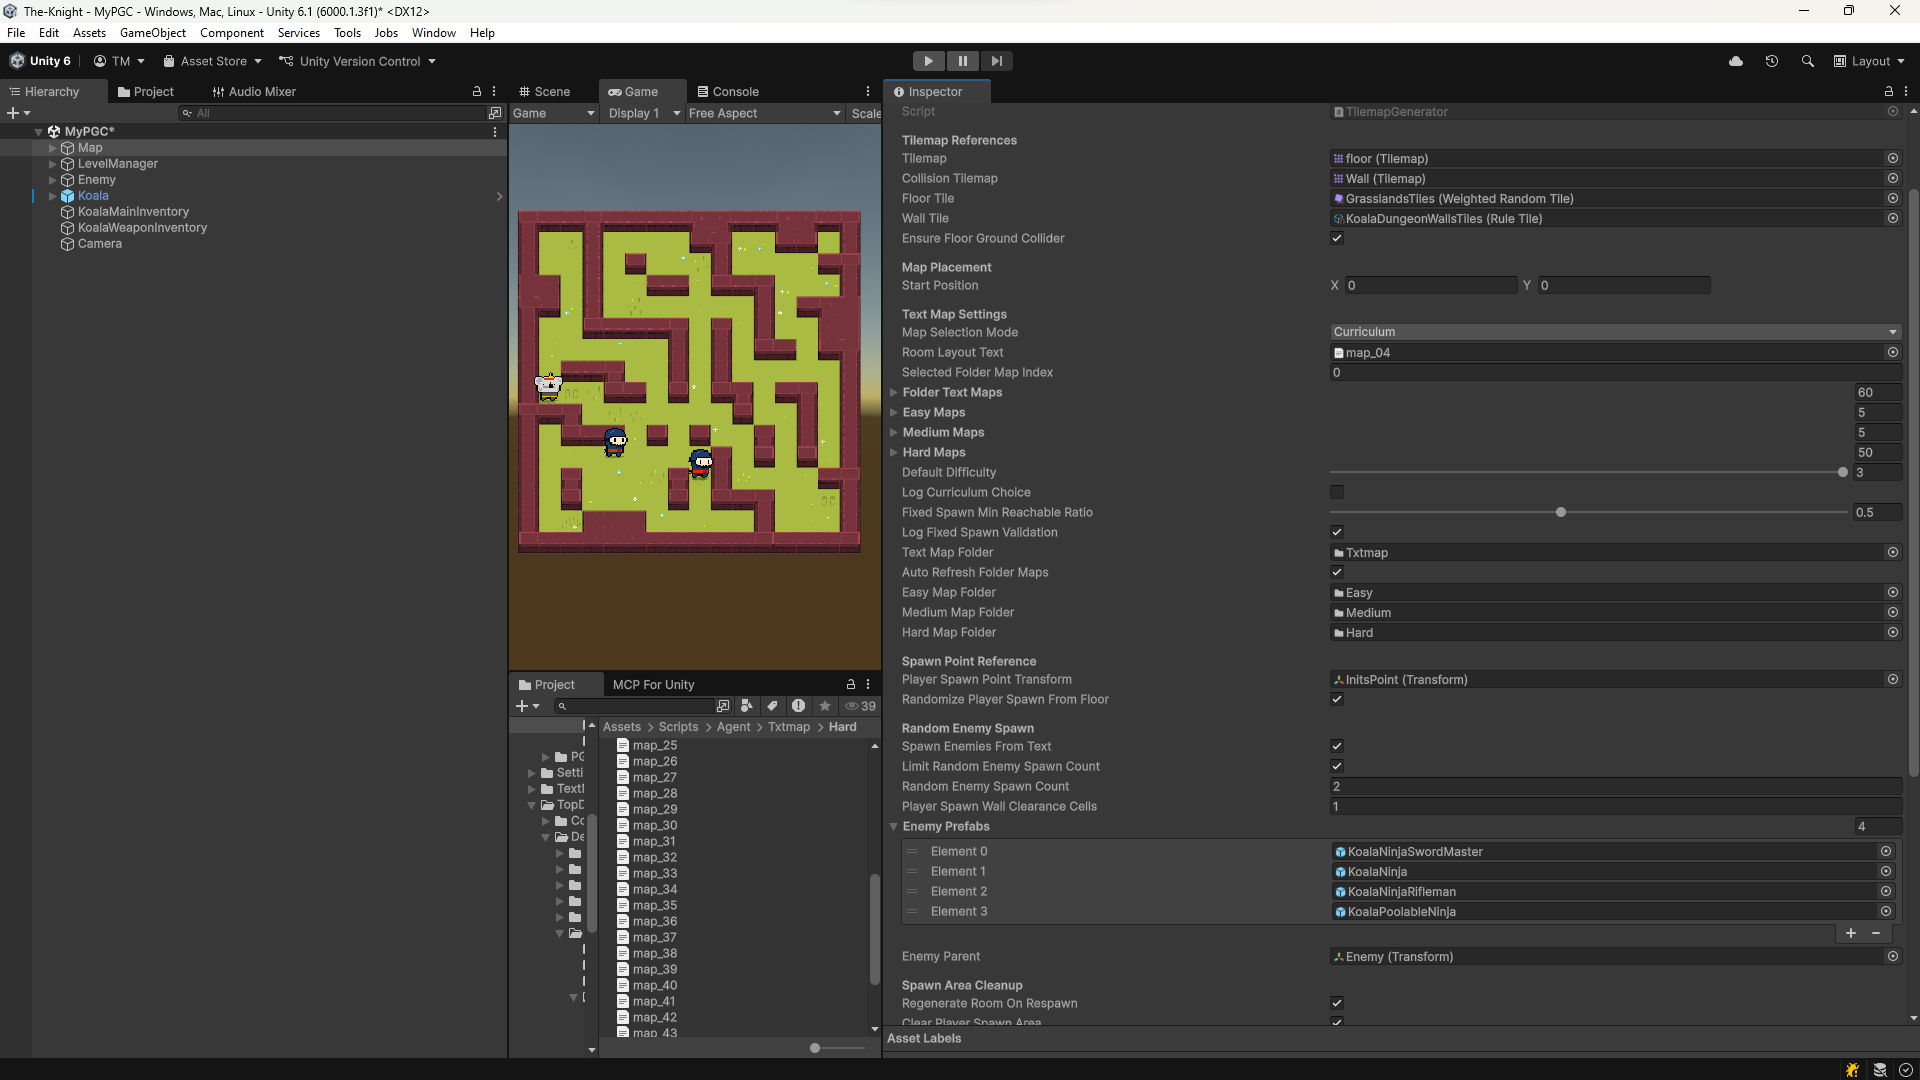
\includegraphics[width=0.98\textwidth]{figures/unity_env.png}
    \caption{Cấu hình TilemapGenerator trong Unity Inspector và ví dụ bản đồ đang được dựng trong Game view}
    \label{fig:unity_tilemap_generator_inspector}
\end{figure}

Bảng~\ref{tab:difficulty_spawn_policy} tóm tắt cách chọn bản đồ và vị trí sinh trong từng mức độ khó. Trong các run curriculum chính, tham số môi trường \emph{difficulty} do ML-Agents truyền vào quyết định cả thư mục bản đồ lẫn chế độ sinh. Với \emph{difficulty}=0, 1 và 2, hệ thống dùng fixed spawn: trên mỗi bản đồ, vị trí người chơi được chọn theo một quy tắc xác định và được lưu tạm, còn các vị trí kẻ địch được chọn từ các ô sàn có thể đi tới từ người chơi, trải theo các mức khoảng cách trung bình để tránh việc kẻ địch luôn xuất hiện quá gần hoặc quá xa. Với \emph{difficulty}=3, hệ thống vẫn dùng tập Hard nhưng chuyển sang random spawn: người chơi và kẻ địch được lấy ngẫu nhiên từ các ô sàn hợp lệ sau mỗi episode. Trong cấu hình huấn luyện chính, số kẻ địch sinh ra mỗi episode được giới hạn bởi \emph{randomEnemySpawnCount}=2; nếu có nhiều prefab enemy, prefab cụ thể được lấy từ mảng \emph{enemyPrefabs}.

\begin{table}[H]
    \centering
    \small
    \caption{Chính sách chọn bản đồ và vị trí sinh theo tham số \emph{difficulty}}
    \label{tab:difficulty_spawn_policy}
    \makebox[\textwidth][c]{%
    \begin{tabular}{|c|p{2.3cm}|p{2.5cm}|p{4.0cm}|p{4.0cm}|}
        \hline
        \textbf{\emph{difficulty}} & \textbf{Nhóm bản đồ} & \textbf{Chế độ sinh} & \textbf{Vị trí sinh người chơi} & \textbf{Vị trí sinh kẻ địch} \\
        \hline
        0 & Easy & Fixed & Một ô sàn hợp lệ được chọn xác định cho từng bản đồ, ưu tiên vùng có không gian di chuyển tốt. & Tối đa 2 kẻ địch ở các ô sàn hợp lệ, có thể đi tới từ người chơi và phân bố ở khoảng cách trung bình. \\
        \hline
        1 & Medium & Fixed & Giữ quy tắc sinh cố định như Easy nhưng dùng tập bản đồ phức tạp hơn. & Giữ quy tắc sinh kẻ địch cố định để giảm phương sai khi tác nhân học bản đồ khó hơn. \\
        \hline
        2 & Hard & Fixed & Dùng tập Hard nhưng vẫn cố định vị trí sinh theo từng bản đồ. & Kẻ địch vẫn được đặt xác định theo bản đồ để tác nhân học kỹ năng chiến đấu trên cấu trúc khó trước. \\
        \hline
        3 & Hard & Random & Chọn ngẫu nhiên một ô sàn hợp lệ ở mỗi episode. & Chọn ngẫu nhiên tối đa 2 ô sàn hợp lệ có thể đi tới từ người chơi, nhằm tăng khả năng khái quát hóa với vị trí sinh mới. \\
        \hline
    \end{tabular}
    }
\end{table}

Như vậy, độ khó không chỉ tăng vì bản đồ chuyển từ Easy sang Medium và Hard, mà còn vì phương sai vị trí sinh được mở rộng ở lesson Hard Random. Cách tách này giúp tác nhân học trước các kỹ năng cơ bản như tiếp cận, né đạn và căn hướng tấn công trong môi trường ít nhiễu hơn, rồi mới phải thích nghi với vị trí sinh thay đổi mạnh.

\section{Khung curriculum learning}

Curriculum learning được dùng để giảm độ khó khám phá ban đầu \cite{Bengio2009}. Thay vì đưa tác nhân ngay vào toàn bộ phân phối Hard, hệ thống bắt đầu từ bản đồ dễ hơn, chuyển sang Medium khi phần thưởng làm mượt vượt ngưỡng, rồi mới chuyển sang nhóm bản đồ Hard. Tham số bài học được truyền qua Academy.Instance.EnvironmentParameters với tên difficulty.

\begin{figure}[H]
    \centering
    \begin{tikzpicture}[>=stealth,
        lesson/.style={draw, rounded corners, align=center, minimum width=3.0cm, minimum height=0.9cm, font=\small},
        transition/.style={font=\scriptsize, fill=white, inner sep=1.5pt}]
        \node[lesson] (easy) at (0,0) {Lesson 0\\Easy};
        \node[lesson] (medium) at (5.0,0) {Lesson 1\\Medium};
        \node[lesson] (hard) at (10.0,0) {Lesson 2\\Hard};
        \node[lesson, minimum width=3.2cm] (random) at (10.0,-1.8) {Lesson 3\\Hard Random};
        \draw[->] (easy.east) -- node[transition, above]{phần thưởng $\geq T_0$} (medium.west);
        \draw[->] (medium.east) -- node[transition, above]{phần thưởng $\geq T_1$} (hard.west);
        \draw[->, dashed] (hard.south) -- node[transition, right]{run54} (random.north);
    \end{tikzpicture}
    \caption{Cấu trúc curriculum 3 bậc và biến thể 4 bậc fixed-to-random}
    \label{fig:curriculum_structure}
\end{figure}

Trong run46, curriculum gồm 3 lesson: Easy, Medium và Hard. Trong run54, curriculum được mở rộng thành 4 lesson: \emph{Easy Fixed}, \emph{Medium Fixed}, \emph{Hard Fixed} và \emph{Hard Random}. Biến thể 4 bậc kiểm tra giả thuyết rằng việc giảm phương sai vị trí sinh ở giai đoạn đầu có thể giúp PPO ổn định hơn trước khi chuyển sang phân phối khó hơn.

Cần phân biệt hai lớp tổ chức độ khó. Lớp thứ nhất là chia tập bản đồ PCGNN thành các thư mục Easy, Medium và Hard dựa trên chỉ số hình học. Lớp thứ hai là lịch chuyển lesson trong ML-Agents: trainer thay đổi tham số \emph{difficulty} khi phần thưởng làm mượt vượt ngưỡng, từ đó TilemapGenerator chọn thư mục bản đồ và chế độ sinh tương ứng.

\section{Kiến trúc mạng và cấu hình PPO}

Chính sách được huấn luyện bằng PPO trong Unity ML-Agents \cite{Juliani2018}. Cấu hình nền dùng mạng MLP actor-critic với hidden\_units=256, num\_layers=2, normalize=true. Actor head sinh phân phối xác suất cho bốn nhánh hành động, còn critic head ước lượng $V(s)$ để tính lợi thế theo GAE.

\begin{figure}[H]
    \centering
    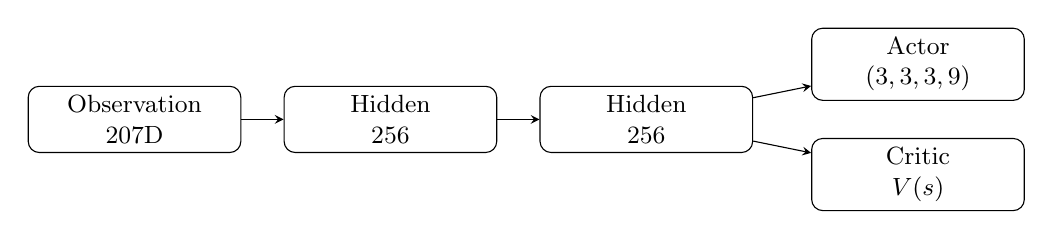
\begin{tikzpicture}[node distance=1.45cm, >=stealth, every node/.style={font=\small}]
        \node[draw, rounded corners, align=center, minimum width=2.7cm] (obs) {Observation\\207D};
        \node[draw, rounded corners, align=center, right of=obs, xshift=1.8cm, minimum width=2.7cm] (h1) {Hidden\\256};
        \node[draw, rounded corners, align=center, right of=h1, xshift=1.8cm, minimum width=2.7cm] (h2) {Hidden\\256};
        \node[draw, rounded corners, align=center, right of=h2, xshift=2.0cm, yshift=0.7cm, minimum width=2.7cm] (actor) {Actor\\$(3,3,3,9)$};
        \node[draw, rounded corners, align=center, right of=h2, xshift=2.0cm, yshift=-0.7cm, minimum width=2.7cm] (critic) {Critic\\$V(s)$};
        \draw[->] (obs) -- (h1);
        \draw[->] (h1) -- (h2);
        \draw[->] (h2) -- (actor);
        \draw[->] (h2) -- (critic);
    \end{tikzpicture}
    \caption{Kiến trúc actor-critic dùng cho CombatAgentConfig}
    \label{fig:actor_critic_architecture}
\end{figure}

Một số run ablation bổ sung bộ nhớ LSTM với memory\_size=256 và sequence\_length=64 để kiểm tra giả thuyết rằng thông tin lịch sử có thể giúp tác nhân xử lý đạn, hồi chiêu và tình huống khuất tầm nhìn. Kết quả định lượng của các lựa chọn kiến trúc này được trình bày ở Chương~4.

Chính sách dùng MLP actor-critic (hidden\_units=256, num\_layers=2, normalize=true). Actor sinh phân phối xác suất cho 4 nhánh hành động; Critic ước lượng $V(s)$ làm baseline cho GAE. Các run LSTM bổ sung memory\_size=256, sequence\_length=64. Các hyperparameter PPO chính (learning\_rate=$3\times10^{-4}$, batch\_size=1024, buffer\_size=10240, num\_epoch=3, $\gamma$=0.99, $\lambda$=0.95, $\epsilon$=0.2, $\beta$=$5\times10^{-3}$) được giữ thống nhất giữa các run ablation run34--run54 để cô lập tác động của từng kỹ thuật. Chi tiết các thay đổi trong run62 được trình bày ở Chương~3.
